%% ----------------------------------------------------------------
%% Prototype.tex
%% ---------------------------------------------------------------- 
\chapter{Prototype of the Forum Visualisation Tool} \label{Chapter:Prototype}

This chapter outlines the specification of \emph{RiskVis}, which is a prototype of the forum visualisation tool. This specification is not intended to be exhaustive and will only focus on the architecture as well as several major modules.

\section{Architecture}

\fref{Figure:07_01} illustrates the high-level architecture of \emph{RiskVis}, which is a standalone desktop application powered by Java Desktop Technologies (Java Swing and Java 2D). It also exploits a host of third party libraries which are rendered in grey in the diagram to execute specific tasks such as the database connection and graph visualisation. Additionally, the database in the left of the diagram is based on PostgreSQL, which contains the relational data model described in Section~\ref{sec:data_model}. Furthermore, the NetBeans Platform is employed as the framework so that it is possible to develop a modular and loosely coupled application that can be easily extended in the future.

\begin{figure}[!htb]
  \centering
  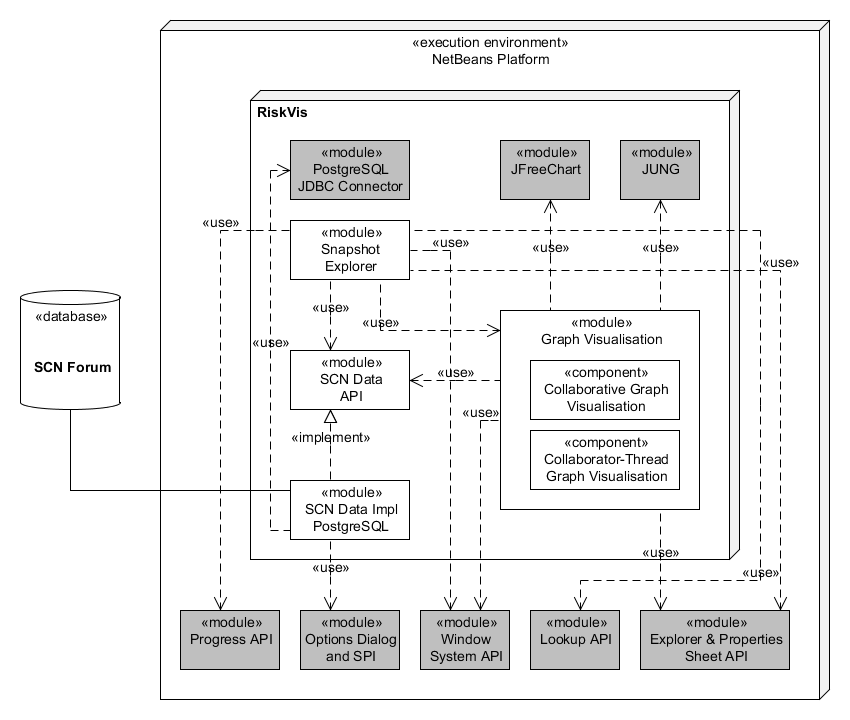
\includegraphics[width=13cm]{07_01_riskvis_architecture}
  \caption{The architecture diagram of \emph{RiskVis}. Rectangles with module label refer to NetBeans modules. Dash arrows with use label refer to dependency between two modules.}
  \label{Figure:07_01}
\end{figure}

\section{NetBeans Platform}

The NetBeans Platform is a generic framework for developing Java Swing applications. \emph{RiskVis} makes use of it as the execution environment for two reasons. Firstly, it provides a complete framework which contains a number of infrastructure facilities ranged from a simple menu bar to a complicated window system, as well as a rich set of advanced Java Swing components (the explorer and properties sheet). As a consequence, more effort can be concentrated on the graph visualisation. Secondly, it also offers a solution to organise the whole application into separated modules. More precisely, a specific module is allowed to call Application Programming Interfaces (APIs) provided by other modules if and only if this caller module has explicitly defined dependencies upon those callee modules. In \fref{Figure:07_01}, the dashed arrows with the use label refer to the dependency between two modules. This section introduces five most relevant NetBeans modules to \emph{RiskVis}, which are outside the application boundary.

\subsection{Lookup API}

The Lookup API provides a way to use the dependency injection so that a module can initialise an object defined in another module without explicitly building dependency between them. This feature will be used in the snapshot explorer module.

\subsection{Window System API}

The Window System API provides a Multiple Document Interface (MDI), which contains functionality such as maximise/minimise, dock/undock, and drag-and-drop of windows. As the building block of \emph{RiskVis}, the snapshot explorer and graph visualisation discussed in the previous chapter will be managed under this window system. \fref{Figure:07_02} presents four windows being displayed simultaneously.

\subsection{Progress API}

The Progress API enables developers to use the progress bar in the bottom right of \fref{Figure:07_02}, to indicate the current progress when executing long-time tasks. This feature will be used in the snapshot explorer module.

\subsection{Explorer \& Properties Sheet API}

The Explorer \& Property Sheet API provides two advanced Java Swing components for displaying data models. The explorer in the left of \fref{Figure:07_02} allows end users to browse hierarchical data in the tree view, whilst the properties sheet in the right of \fref{Figure:07_02} displays the detailed information about an item in the tree view. This feature will be used in the snapshot explorer and graph visualisation module, which efficiently present objects defined in the enhanced data model (see \fref{Figure:06_09}).

\begin{figure}[!htb]
  \centering
  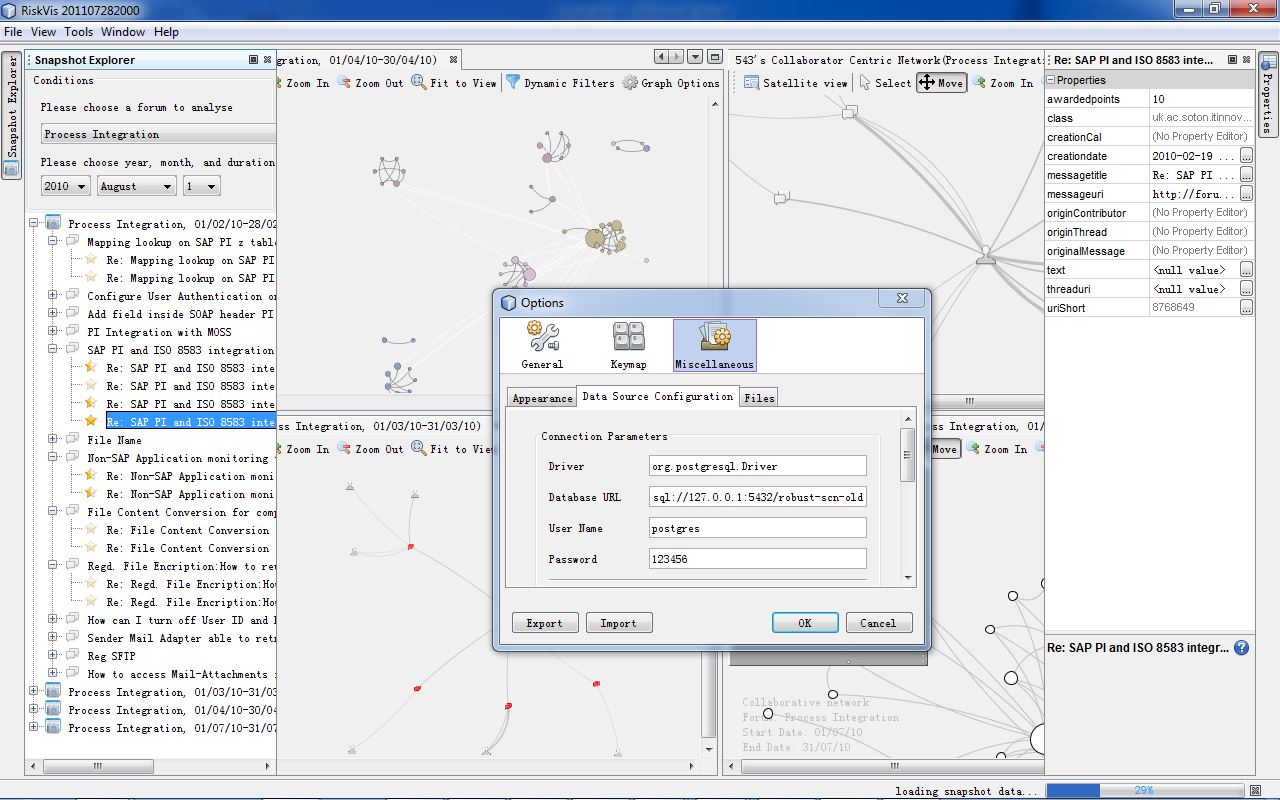
\includegraphics[width=14cm]{07_02_riskvis_screenshot}
  \caption{The screenshot presents several major feature of \emph{RiskVis} powered by NetBeans Platform, including multiple windows, progress bar in the bottom right, explorer window in the left, the properties sheet window in the right, and the global options dialogue in the centre.}
  \label{Figure:07_02}
\end{figure}

\subsection{Options and Dialogue SPI}
The Options and Dialogue SPI provides a way to integrate with the global options window in the centre of \fref{Figure:07_02} so that end users can customise the application. This feature will be used in the SCN Data Implementation module.

\section{RiskVis Module Description} \label{sec:riskvis_module_desc}

\emph{RiskVis} is made up of seven modules: the Snapshot Explorer, Graph Visualisation, SCN Data API, SCN Data Implementation, JUNG, JFreeChart, and PostgreSQL JDBC Connector. The last three modules are wrapper library modules that contain no code but the corresponding libraries: the PostgreSQL driver to connect to the SCN Forum database, the JUNG library as the graph visualisation framework discussed in Section~\ref{sec:evaluation_vis_framework}, and the chart library to draw temporal bar charts in the collaborator-thread graph visualisation (see \fref{Figure:06_18}), respectively. The section presents the other four modules in more technical details.

\subsection{SCN Data API}

As illustrated in \fref{Figure:07_03}, the SCN Data API module implements the enhanced data model (see \fref{Figure:06_09}) in the entity package. It also defines generic data access APIs in the \emph{SnapshotService} interface to get forums, threads, and messages from the data source in the form of the Java interface.

\begin{figure}[!htb]
  \centering
  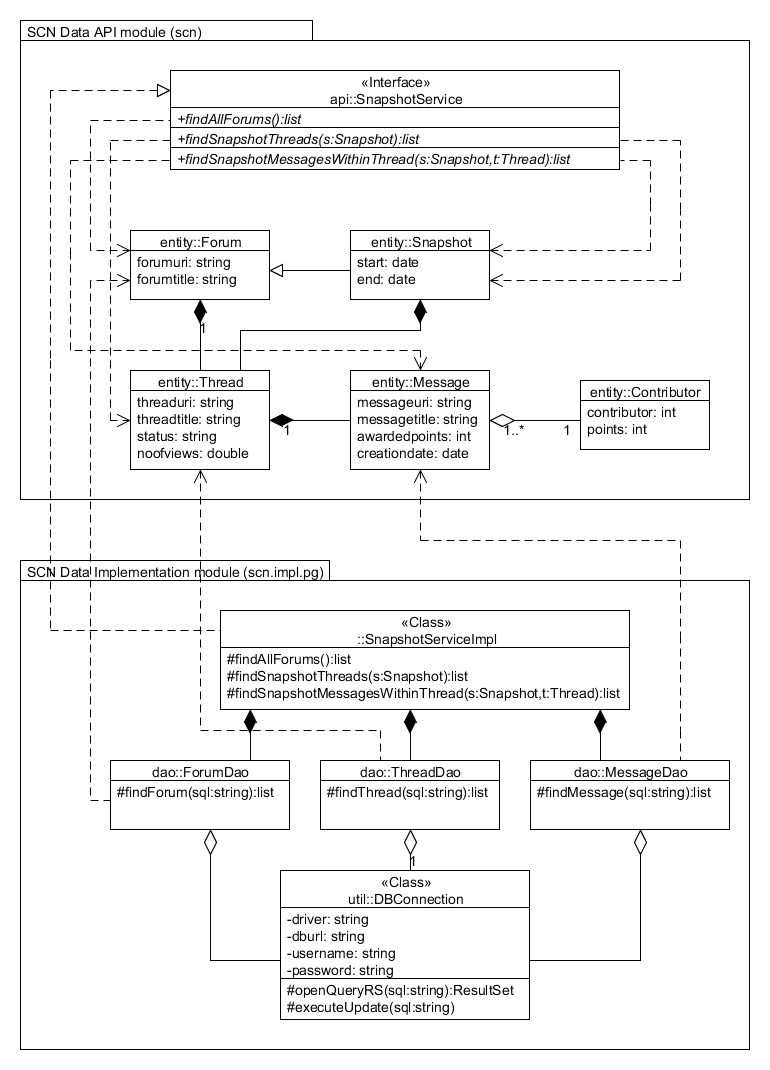
\includegraphics[width=13cm]{07_03_scn_data_class_diagram}
  \caption{The class diagram including SCN Data API module and SCN Data Implementation module.}
  \label{Figure:07_03}
\end{figure}

\subsection{SCN Data Implementation}

\fref{Figure:07_03} also shows the detailed structure of the SCN Data Implementation module, which consists of the Data Access Object (DAO) package and default package. The former is designed for accessing database as a set of low-level data manipulation classes. The latter implements the \emph{SnapshotService} interface defined in the SCN Data API module by using the DAO package. Additionally, this module also includes the \emph{DBConnection} class which provides a user interface for end users to configure the database connection parameters such as the database URL, username, and password. With the aid of the Options and Dialogue SPI module, this feature has been integrated into the global options dialogue.

\subsection{Snapshot Explorer}

As the starting point of \emph{RiskVis}, the snapshot explorer module includes the condition panel (see \fref{Figure:06_11}) which allows end users to load data in any user-specified snapshot. The Lookup API is used to get an instance of the \emph{SnapshotService} interface defined in the SCN Data API module, although there is no dependency upon the SCN data Implementation module that has really provided an implementation (the \emph{SnapshotServiceImpl} class) of the interface. The benefit of this loosely coupled strategy is that any other SCN Data implementation can easily take over without any modification to the modules that use the SCN data.

As discussed in Section~\ref{sec:requirements}, the load action will be executed in the background thread with conveying the progress of the task powered by the Progress API. In this way, end users are allowed to interact with an existing snapshot when waiting for data being loaded. Once the data has been successfully loaded from the database, the new hierarchical data in the form of snapshot-thread-message is expected to be added into the tree view. Meanwhile, the collaborative graph visualisation will be automatically opened by the window system.

Additionally, it is important to note that the snapshot explorer window in this module is considered as a singleton component under the management of the window system.

\subsection{Graph Visualisation}

The graph visualisation module is the most important module of the application, which is made up of three packages: the collaborative graph visualisation, collaborator-thread graph visualisation, and utility package. \fref{Figure:07_04} presents the simple class diagram of this module, which will not be specified down to the smallest detail but from the high-level perspective.

The collaborative graph visualisation package consists of three visual components: the \emph{CollaborativeTopComponent}, \emph{CollaborativeFiltersComponent}, and \emph{CollaborativeOptionsTopComponent} class, which represent the main window (Section~\ref{sec:collaborative_graph_main_window}), dynamic filters window (Section~\ref{sec:collaborative_graph_filters_window}), and graph options window (Section~\ref{sec:collaborative_graph_options_window}), respectively. Similarly, the collaborator-thread graph visualisation consists of two visual components: the \emph{CollaboratorTopComponent}, and \emph{CollaboratorTemporalTopComponent}, which refer to the main window (\ref{sec:c_t_graph_main_window}) and temporal chart window (\ref{sec:c_t_graph_temporal_chart_window}), respectively.

The utility package provides infrastructure facilities to both graph visualisations. For example, the \emph{ClusterUtil} class makes use of the \emph{WeightedGirvanNewmanAlgorithm} class to encapsulate the cluster finding features described in Section~\ref{sec:collaborative_graph_options_window}. The \emph{GraphUtil} class calculates widely-used metrics such as degree centrality, betweenness centrality, and so forth. The \emph{PopupGraphMousePlugin} class allows end users to open the context menu when right clicking a specific element in the graph visualisation.

\begin{figure}[!htb]
  \centering
  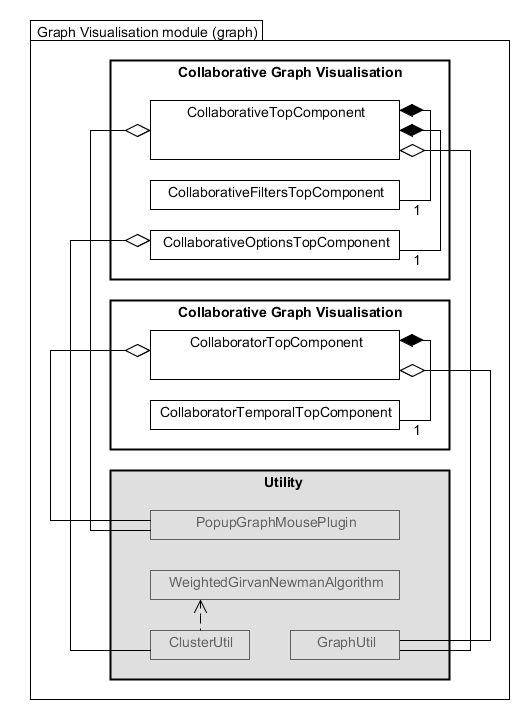
\includegraphics[width=13cm]{07_04_graph_visualisation_class_diagram}
  \caption{The simple class diagram of the graph visualisation module.}
  \label{Figure:07_04}
\end{figure}

\section{Summary}

This chapter briefly summarises the implementation details of \emph{RiskVis} from a modular point of view. All functionalities defined in the previous chapter have been encapsulated within separate modules running in the NetBeans Platform. After an introduction of the application architecture, both the modules provided by NetBeans and those module included in \emph{RiskVis} have been described with class diagrams.
